\begin{document}

\section{Baseline Implementations}

We compare patX against a comprehensive suite of time series analysis methods,
ranging from feature engineering to deep learning and state-of-the-art ensembles.
For feature-based methods (patX, tsfresh, catch22, MiniRocket, RDST), we train a
LightGBM classifier on the extracted features. CNN is trained end-to-end.

\subsection{tsfresh}
\textbf{tsfresh} \cite{christ2018tsfresh} extracts a massive library of
statistical and spectral characteristics. We use \texttt{MinimalFCParameters} to
balance coverage and feature count.

\subsection{catch22}
\textbf{catch22} \cite{lubba2019catch22} provides a canonical set of 22
computationally efficient time series features.

\subsection{MiniRocket}
\textbf{MiniRocket} \cite{dempster2021minirocket} is a state-of-the-art
method transforming signals via $\sim$10,000 random convolutional kernels.
It represents the ``accuracy-at-all-costs'' end of the spectrum, offering high
performance but low interpretability.

\subsection{RDST}
\textbf{RDST} \cite{guillaume2022random} (Random Dilated Shapelet Transform) is a
fast and accurate shapelet-based approach that introduces dilation to capture
patterns at multiple scales with improved computational efficiency.

\subsection{CNN}
\textbf{CNN}: A 1D Convolutional Neural Network trained end-to-end, representing
the deep learning baseline. We implement a 1D CNN using PyTorch with three
convolutional layers (filters: 64, 128, 256) each containing convolution, batch
normalization, ReLU, max pooling, and dropout. The architecture uses kernel sizes
of 7, 5, and 3 for the three layers respectively, with appropriate padding to
maintain temporal resolution. Adaptive average pooling aggregates features across
the temporal dimension, followed by fully connected layers (256→128→64→output)
with ReLU activations, batch normalization, and dropout (0.4, 0.3) for
regularization. We train with Adam optimizer (lr=0.1, weight decay=1e-4), early
stopping (patience=10), and learning rate reduction on plateau (factor=0.5,
patience=3). For binary classification tasks, we use cross-entropy loss with
class weights computed to handle imbalanced datasets; for multi-class
classification and regression, we use unweighted cross-entropy and MSE loss
respectively. The model automatically detects the number of input channels based
on the dataset structure: 3 channels for AZT1D (CGM, insulin, carbs), 5 channels
for REMC (histone marks), and 1 channel for univariate time series. Training
uses 100 epochs maximum with batch size 128, matching evaluation protocols with
other baselines.

\section{Dataset Processing Details}

\subsubsection{AZT1D Preprocessing: Insulin and Carbohydrate Response Modeling}

The AZT1D dataset presents unique challenges for glucose forecasting due to the
complex temporal dynamics of insulin and carbohydrate effects on blood glucose
levels.
Unlike simple time series where immediate effects are observed, physiological
responses involve significant delays: insulin takes 10--90 minutes to affect
glucose levels, while carbohydrates impact glucose within 10--60 minutes, with
effects persisting for 2--4 hours \cite{woldaregay2019data}.

To address these delayed physiological responses, we implement knowledge-driven
response curve modeling based on established pharmacokinetic and glycemic
response literature.
For insulin, we use a gamma-like function with 15-minute onset, 60-minute peak,
and 4-hour duration; for carbohydrates, we use 10-minute onset, 45-minute peak,
and 3-hour duration.
These response curves model the temporal dynamics of physiological effects, with
insulin effects peaking around 60 minutes and persisting for up to 4 hours,
while carbohydrate effects peak around 45 minutes and persist for up to 3 hours.

At each timepoint, we compute cumulative active effects by convolving all
historical insulin doses and carbohydrate intakes with their respective response
curves.
This creates interpretable time series that capture overlapping physiological
effects, enabling the model to understand how multiple insulin doses and meal
intakes interact over time.

The preprocessing pipeline extracts 24 timepoints (2 hours of history at
5-minute intervals) for three physiological signals: CGM values, active insulin
effects, and active carbohydrate effects.
The regression target is future glucose change $g_{t+h} - g_t$ where
$h = 30$ minutes (6 timepoints ahead).
We also include the initial CGM value (CGM\_0) as a baseline feature to provide
current glucose context.

\begin{figure}[H]
  \centering
  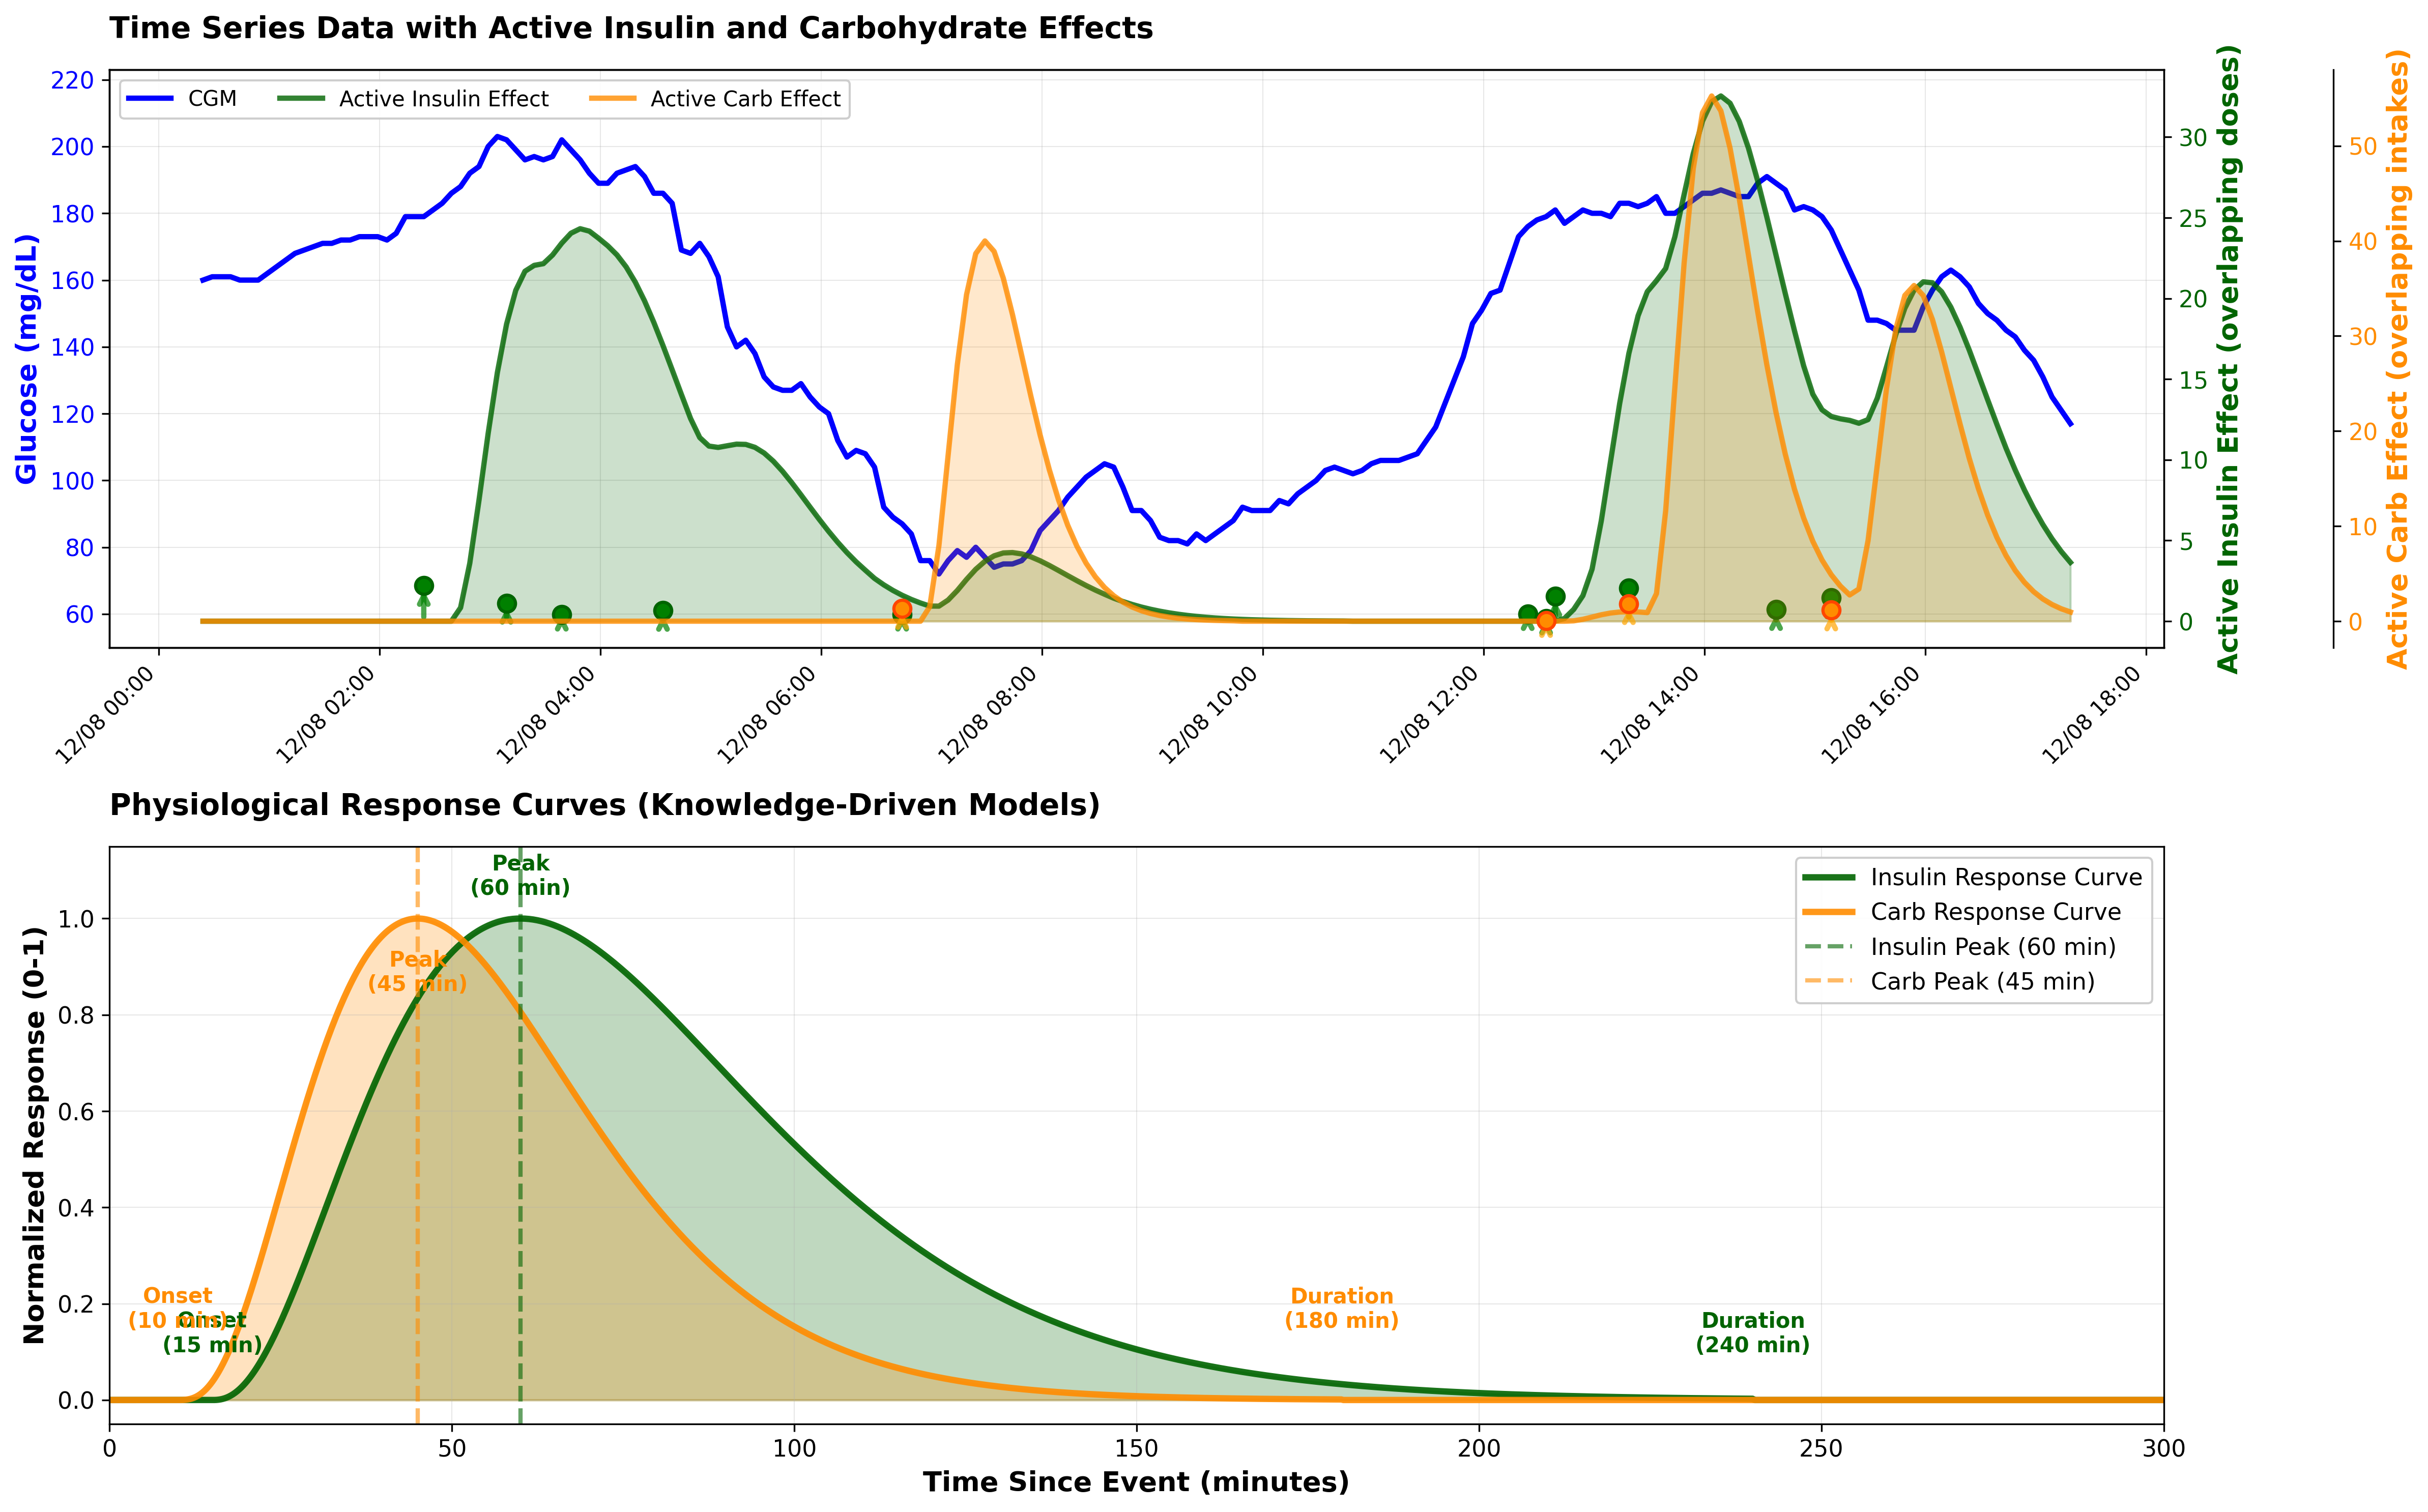
\includegraphics[width=\textwidth,keepaspectratio]{images/supplementary/azt1d_insulin_carb_visualization.png}
  \caption{AZT1D preprocessing visualization showing insulin and carbohydrate
  response modeling.
  Top panel: Real-time CGM with overlapping insulin and carbohydrate effects
  over time for Subject 1.
  Blue line shows CGM values with target range (70-180 mg/dL) highlighted in
  green.
  Dark green shaded area represents active insulin effect from overlapping
  doses (circles with crosses).
  Orange shaded area represents active carbohydrate effect from overlapping
  intakes (circles with crosses).
  Bottom panel: Physiological response curves showing normalized insulin
  (15-min onset, 60-min peak, 240-min duration) and carbohydrate (10-min onset,
  45-min peak, 180-min duration) effects over time.
  These knowledge-driven models enable patX to learn from physiologically
  meaningful features that capture delayed and overlapping effects.}
  \label{fig:azt1d_preprocessing}
\end{figure}

This preprocessing approach transforms raw event data into continuous
physiological signals that capture the complex temporal dynamics of glucose
regulation, providing patX with meaningful features for pattern discovery across
multiple signal representations.

\subsubsection{MITBIH Preprocessing}

The MIT-BIH Arrhythmia Database contains annotated ECG recordings from 48 patients.
We extract individual heartbeats by centering 100-sample windows around annotated
R-peak positions, with 50 samples before and 50 samples after each R-peak.
Each beat is classified into one of five arrhythmia types: Normal (N), Left bundle
branch block (L), Right bundle branch block (R), Atrial premature (A), and
Premature ventricular contraction (V).
To address class imbalance, we apply random undersampling to balance class
distributions before training.

\begin{figure}[H]
  \centering
  
\includegraphics[width=0.6\textwidth,keepaspectratio]
  {images/supplementary/mitbih_sample.png}
  \caption{Representative ECG beat from MITBIH dataset showing characteristic
  R-peak morphology.}
  \label{fig:mitbih_sample}
\end{figure}

\subsubsection{Emotions Preprocessing}

The EEG emotions dataset contains brainwave recordings collected while participants
experienced different emotional states (positive, neutral, negative).
We extract FFT-derived features from 5 EEG channels (AF3, F7, F3, FC5, T7), yielding 254 frequency bins per channel.
The FFT features are organized into two groups (a and b suffixes) representing
different frequency decomposition components, providing 5 input channels with 254
time points each for pattern discovery.

\begin{figure}[H]
  \centering
  
\includegraphics[width=0.6\textwidth,keepaspectratio]
  {images/supplementary/emotions_sample.png}
  \caption{Representative EEG frequency spectra from Emotions dataset showing
  power distributions across five channels.}
  \label{fig:emotions_sample}
\end{figure}

\subsubsection{REMC Preprocessing}

Following our prior work on PatternChrome \cite{paul2025prediction}, we predict
binary gene expression (high/low) from histone modification ChIP-seq profiles from
the Roadmap Epigenomics Consortium (56 cell lines, 19,795 genes).
We convert RefSeq to GENCODE identifiers, retaining 18,421 genes.
For each gene, we extract five histone modification signals (H3K4me1, H3K4me3,
H3K36me3, H3K9me3, H3K27me3) from 5000 bp upstream and downstream of the TSS,
divided into 50 bp bins (200 bins per mark).
Gene expression is binarized at the median level.
We split 6,600/5,911/5,910 genes for train/validation/test with balanced labels.

\begin{figure}[H]
  \centering
  
\includegraphics[width=0.6\textwidth,keepaspectratio]
  {images/supplementary/remc_sample.png}
  \caption{Representative histone modification profiles from REMC dataset showing
  all five marks (H3K4me3, H3K4me1, H3K36me3, H3K9me3, H3K27me3) around the
  transcription start site for a high-expression gene.}
  \label{fig:remc_sample}
\end{figure}

\subsubsection{MIMIC-IV Preprocessing}

We predict ARDS from multivariate clinical time series in ICU patients.
The dataset contains 29 features per subject: vital signs (respiratory rate,
heart rate, O2 saturation, blood pressure, temperature), ventilator settings
(FiO2, PEEP), Glasgow Coma Scale scores, laboratory values (arterial pH, PaO2,
creatinine, platelets, WBC, INR, lactate, bilirubin), vasopressors (norepinephrine,
phenylephrine, epinephrine, dopamine, dobutamine), urine output, and derived
features (PaO2/FiO2 ratio, pulse pressure).
We extract 24-hour time series binned hourly, with forward/backward filling for
missing values and 0.1/99.9th percentile capping for extreme values.
Subjects with $<$5 hours of data are excluded; anchor\_age is provided as baseline.

\begin{figure}[H]
  \centering
  
\includegraphics[width=0.6\textwidth,keepaspectratio]
  {images/supplementary/mimic_sample.png}
  \caption{Representative clinical time series from MIMIC-IV dataset showing
  24-hour trajectories of vital signs, laboratory values, and ventilator settings.}
  \label{fig:mimic_sample}
\end{figure}

\subsubsection{PAMAP2 Preprocessing}

The PAMAP2 dataset contains recordings from 9 subjects performing 18 physical
activities while wearing 3 IMUs (wrist, chest, ankle) and a heart rate monitor.
Each IMU records temperature, 3D acceleration ($\pm$16g and $\pm$6g scales),
3D gyroscope, 3D magnetometer, and 4D orientation at 100Hz, yielding 51 channels.
We create 100-sample windows (1 second) with 50\% overlap, filtering transient
activities (ID 0) to obtain 12 activity classes: lying, sitting, standing, walking,
running, cycling, Nordic walking, watching TV, computer work, ascending/descending
stairs, and vacuum cleaning.
Missing values are interpolated and filled with column means.

\begin{figure}[H]
  \centering
  
\includegraphics[width=0.6\textwidth,keepaspectratio]
  {images/supplementary/pamap2_sample.png}
  \caption{Representative IMU sensor data from PAMAP2 dataset showing
  acceleration and gyroscope measurements from hand, chest, and ankle sensors.}
  \label{fig:pamap2_sample}
\end{figure}

\subsubsection{SVD Preprocessing}

The Saarbr\"ucken Voice Database (SVD) contains voice recordings from over 2000
subjects, including healthy controls and patients with 71 different voice
pathologies \cite{lee2021experimental}.
Following the exact methodology of Lee \cite{lee2021experimental}, we select
balanced subsets for male and female subjects separately:
\begin{itemize}
\item \textbf{Female}: 259 healthy + 259 pathological (97 hyperfunctional
      dysphonia, 51 functional dysphonia, 30 laryngitis, 81 other)
\item \textbf{Male}: 259 healthy + 259 pathological (62 laryngitis,
      44 hyperfunctional dysphonia, 25 vocal fold polyp, 128 other)
\end{itemize}

We extract sustained vowel recordings of /a/, /i/, and /u/ at normal pitch
and apply the following preprocessing pipeline:
(1) bandpass filtering (80--4000~Hz) to remove DC offset and high-frequency
noise, (2) pre-emphasis with coefficient 0.97 to amplify higher frequencies,
(3) silence trimming using RMS-based voice activity detection,
(4) truncation to 3 seconds maximum, and
(5) resampling to 700 samples using polyphase filtering.
Each waveform is normalized to zero mean and unit variance, then clipped to
$\pm5$ standard deviations.

Following Lee \cite{lee2021experimental}, we perform separate evaluations by
gender and vowel to account for physiological differences in fundamental
frequency and vocal tract characteristics between men and women.

\begin{figure}[H]
  \centering
  
\includegraphics[width=0.6\textwidth,keepaspectratio]
  {images/supplementary/svd_sample.png}
  \caption{Representative waveforms from SVD dataset showing preprocessed
  audio signals for sustained vowels /a/, /i/, and /u/ at normal pitch.
  Each vowel is resampled to 700 samples after bandpass filtering and
  silence trimming.}
  \label{fig:svd_sample}
\end{figure}

\end{document}